\section{Government}
	\subsection{Registration}
	The government cannot register a new account like citizens and 
	businesses because only one account is allowed. This account is provided 
	by the developer of \textit{Soldino}.
	\subsection{Login}
	If you want to log on the Government account press the "login" button on the 
	top right of the homepage, you will automatically log in your account 
	(there is no need for a username or password, all is done via MetaMask). 
	\\To be able to log in make sure you are logged in the correct MetaMask\glosp 
	account.
	\subsection{Logout}
	To log out of \textit{Soldino} you just have to log out of 
	MetaMask\glosp. To do this you have to press MetaMask's icon on the top 
	right of the browser, press your account's icon and then press "Log out"
	on the top right.
	\begin{figure}[H]
		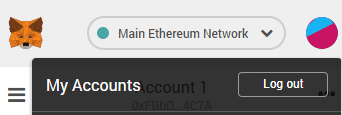
\includegraphics[width=7cm]{res/images/logout_metamask.png}
		\centering
		\caption{Logging out}
	\end{figure}
\pagebreak
	\subsection{Cubit}
	The Government can mint and distribute Cubits\glosp by pressing the "Cubit 
	Manager" button in the navigation bar at the top of the page.
	\begin{figure}[H]
		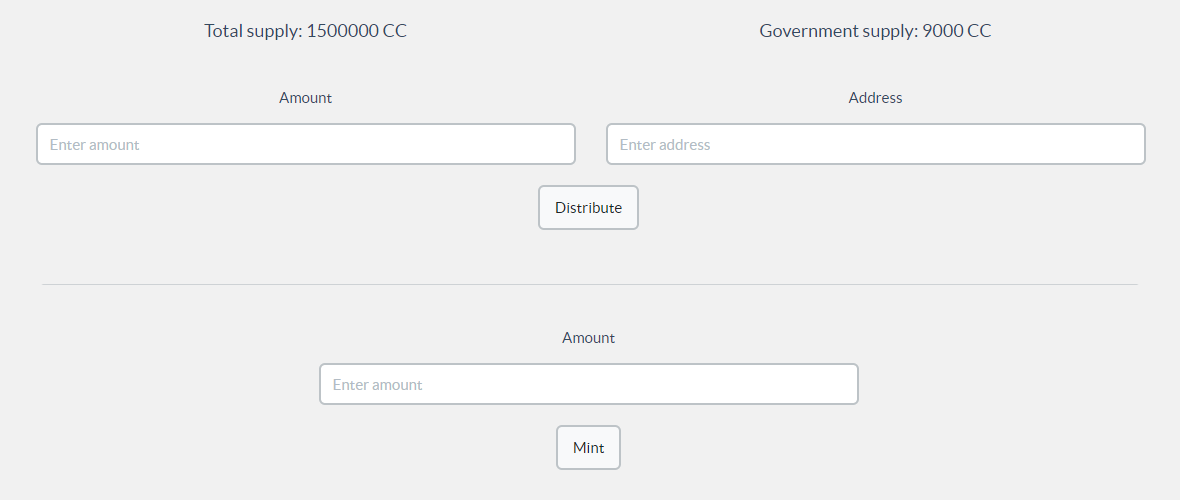
\includegraphics[width=15cm]{res/images/cubit_mint.png}
		\centering
		\caption{Goverment Cubit page}
	\end{figure}
		\subsubsection{Minting}
		To mint Cubits\glosp you have to insert the quantity you want in the 
		"Amount" field at the bottom of the page then press "Mint". You will 
		now see that the "Government supply" is increased by the chosen amount.
		\begin{figure}[H]
			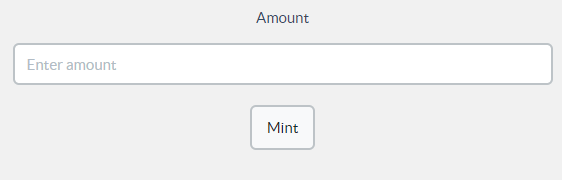
\includegraphics[width=10cm]{res/images/minting_cubits.png}
			\centering
			\caption{Minting Cubits}
		\end{figure}
		\subsubsection{Distributing}
		To distribute Cubits\glosp you have to insert the amount in the "Amount" 
		field, insert the address of the account you wish to send the Cubits to 
		in the "Address" field then press "Distribute".\\
		Remember that this address is not the physical address of the user but 
		their address on the Ethereum\glosp network.
		\begin{figure}[H]
			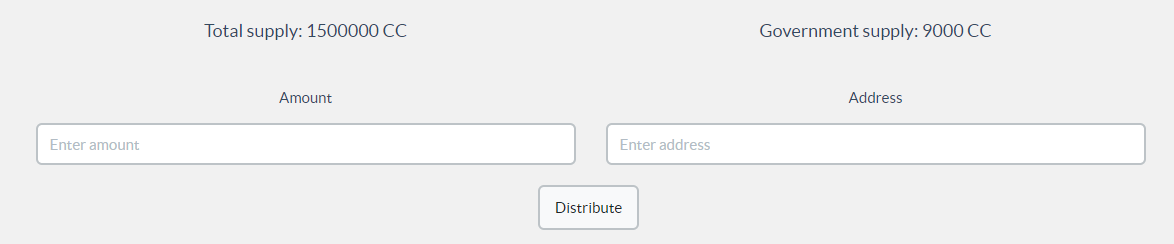
\includegraphics[width=15cm]{res/images/distribute_cubit.png}
			\centering
			\caption{Distributing Cubits}
		\end{figure} \mbox{}\\
		\noindent Note that the amount of cubit must be lower than the "Government  
		supply" otherwise you will not be able to send them.
	\subsection{Managing users}
	The Government can activate disabled accounts or deactivate active accounts.
	This can be done by clicking on the "Users List" button in the navigation
	bar at the top of the page. Here you will find all users registered in 
	\textit{Soldino} with all their information.
	\begin{figure}[H]
		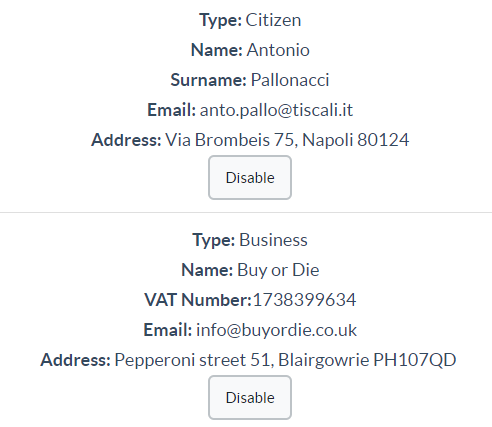
\includegraphics[width=13cm]{res/images/users_list.png}
		\centering
		\caption{Example of users list}
	\end{figure}
		\subsubsection{Deactivating users}
		After you have found the account you want to disable press the 
		"Disable" button. Disabling an account means that it will not be able to make purchases on \textit{Soldino} 
		until it is enabled.
		\begin{figure}[H]
			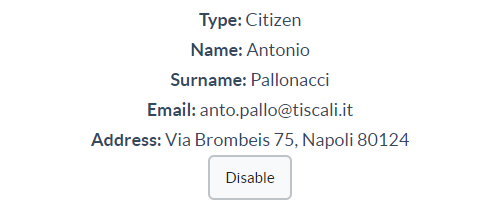
\includegraphics[width=13cm]{res/images/users_disable.png}
			\centering
			\caption{Example of disabling an activated account}
		\end{figure}
		\subsubsection{Activating users}
		After you have found the account you want to enable press the button 
		"Enable". After being enabled an account will again be able to make 
		purchases on \textit{Soldino}.
		\begin{figure}[H]
			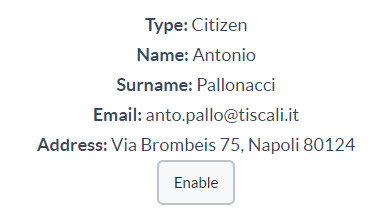
\includegraphics[width=10cm]{res/images/user_enable.png}
			\centering
			\caption{Example of enabling a deactivated account}
		\end{figure}
	\subsection{Refund VAT}
	To refund businesses of their VAT output you have to press the "VAT 
	Refund" button in the navigation bar at the top of the page, in the 
	page that loads you will find all businesses with VAT output for the current quarter.
	Press "Refund" to refund the selected business.
	\begin{figure}[H]
		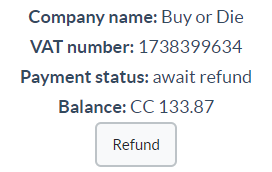
\includegraphics[width=7cm]{res/images/business_refund.png}
		\centering
		\caption{Example of reimbursing a business}
	\end{figure}